% Exam Template for UMTYMP and Math Department courses
%
% Using Philip Hirschhorn's exam.cls: http://www-math.mit.edu/~psh/#ExamCls
%
% run pdflatex on a finished exam at least three times to do the grading table on front page.
%
%%%%%%%%%%%%%%%%%%%%%%%%%%%%%%%%%%%%%%%%%%%%%%%%%%%%%%%%%%%%%%%%%%%%%%%%%%%%%%%%%%%%%%%%%%%%%%

% These lines can probably stay unchanged, although you can remove the last
% two packages if you're not making pictures with tikz.
\documentclass[addpoints,11pt]{exam}
\RequirePackage{amssymb, amsfonts, amsmath, latexsym, verbatim, xspace, setspace}
\RequirePackage{tikz, pgflibraryplotmarks}

% By default LaTeX uses large margins.  This doesn't work well on exams; problems
% end up in the "middle" of the page, reducing the amount of space for students
% to work on them.
\usepackage[margin=1in]{geometry}
\usepackage{multicol}
\usepackage{multirow}


% Here's where you edit the Class, Exam, Date, etc.
\newcommand{\class}{CPSC 6300-002}
\newcommand{\term}{Fall 2019}
\newcommand{\examnum}{Final Exam}
\newcommand{\examdate}{12/12/19}
\newcommand{\timelimit}{150 Minutes}

% For an exam, single spacing is most appropriate
\singlespacing
% \onehalfspacing
% \doublespacing

% For an exam, we generally want to turn off paragraph indentation
\parindent 0ex

\begin{document}

% These commands set up the running header on the top of the exam pages
\pagestyle{head}
\firstpageheader{\class}{\examnum\ - Page \thepage\ of \numpages}{\examdate}
\runningheader{\class}{\examnum\ - Page \thepage\ of \numpages}{\examdate}
\runningheadrule

%\begin{flushright}
%\begin{tabular}{p{2.8in} r l}
%\textbf{\class} & \textbf{Name (Print):} & \makebox[2in]{\hrulefill}\\
%\textbf{\term} &&\\
%\textbf{\examnum} &&\\
%\textbf{\examdate} &&\\
%\textbf{Time Limit: \timelimit} & Teaching Assistant & \makebox[2in]{\hrulefill}
%\end{tabular}\\
%\end{flushright}
%\rule[1ex]{\textwidth}{.1pt}

\begin{coverpages}

\begin{center}
  \textbf{\large{
  Clemson University\\
  School of Computing\\
  CPSC6300 Section 002 - Applied Data Science\\
  Final Exam on December 12, 2019\\
  Duration: 2.5 hours (7:00PM-9:30PM)}}
\end{center}


\textbf{Honor Policy}.

\begin{itemize}
  \item For this exam, you must \textbf{work independently}. You may not aid or accept aid from other students in any means.
  \item During the exam, you may consult two pages of double-sided notes which you have prepared before the exam. However, you must not consult any other paper or online materials.
  \item You are allowed to use a battery-powered calculator in the exam. However, you are not allowed to use the calculators on a smart phone, a laptop, or any other types of mobile devices that is not exclusively designed for calculator purpose.
\end{itemize}

\textbf{Directions}.

\begin{enumerate}
  \item There are 18 pages total (including this page) in this exam. Check if you have all the pages.
  \item Answer the questions on the exam pages in the space provided. You may use the back of the pages for scratch work but final answer must be in the provided spaces.
  \item Read questions carefully and answer as neatly, clearly and concisely as possible; illegible or incomprehensible answers will not get any point.
  \item Should a question be unclear or ambiguous, make a reasonable interpretation and state what you have assumed before answering.
  \item Partial credit will be given for clear formulations of how to solve the problems.
  \item Mysterious or unsupported answers will not receive full credit.
  \item Answer all the questions, including all sub-parts.
\end{enumerate}
\vspace{0.1in}

\makebox[\textwidth]{Last Name:\enspace\hrulefill}
\vspace{0.1in}

\makebox[\textwidth]{First Name:\enspace\hrulefill}
\vspace{0.1in}

\makebox[\textwidth]{Signature:\enspace\hrulefill}
\vspace{0.2in}

\gradetablestretch{2}
\vqword{Problem}
\addpoints % required here by exam.cls, even though questions haven't started yet.	
\gradetable[h]%[pages]  % Use [pages] to have grading table by page instead of question



\end{coverpages}
\newpage % End of cover page

%%%%%%%%%%%%%%%%%%%%%%%%%%%%%%%%%%%%%%%%%%%%%%%%%%%%%%%%%%%%%%%%%%%%%%%%%%%%%%%%%%%%%
%
% See http://www-math.mit.edu/~psh/#ExamCls for full documentation, but the questions
% below give an idea of how to write questions [with parts] and have the points
% tracked automatically on the cover page.
%
%
%%%%%%%%%%%%%%%%%%%%%%%%%%%%%%%%%%%%%%%%%%%%%%%%%%%%%%%%%%%%%%%%%%%%%%%%%%%%%%%%%%%%%
%\qformat{\textbf{Problem \thequestion}\quad (\thepoints) \hfill}
\begin{questions}


% Basic question
\addpoints
\question[15] \textbf{Multiple choices question}. Choose the best answer for each question.

\noaddpoints

\begin{parts}

\part A hospital is building a new care unit for elderly patients. In order to streamline their services, the hospital administration is trying to place patients with similar medical conditions into rooms on the same floor. Overwhelmed with the amount of medical data that is available for each patient, they ask for your help to identify patient groups. What learning problem do you consider this problem to be?

\begin{oneparchoices}
    \choice Supervised learning\\
    \choice Classification\\
    \choice Regression\\
    \choice Clustering\\
    \choice PCA
\end{oneparchoices}

\part A consulting company collects data on the top 500 firms in the US. For each firm they record CEO
salary, profit, number of employees, and industry. They ask you to build a data science model that
explains CEO salary. What learning problem do you consider this task to be?

\begin{oneparchoices}
    \choice Semi-supervised learning\\
    \choice Classification\\
    \choice Regression\\
    \choice Clustering\\
    \choice PCA
\end{oneparchoices}

\part Which of the following metrics is most appropriate for linear model selection?

\begin{oneparchoices}
    \choice $R^2$\\
    \choice Training MSE\\
    \choice $t$-statistic\\
    \choice Mallow's $C_p$\\
    \choice $z$-statistic
\end{oneparchoices}

\part What does \textbf{\emph{F}-Statistic} measure?

\begin{oneparchoices}
 \choice The variability explained by the model.\\
 \choice The variability left unexplained by the model.\\
 \choice The variability explained by the model normalized by the number of predictors.\\
 \choice The ratio of variability explained by the model to the variability left unexplained by the model. \\
 \choice The statistically significance of a single variable.
\end{oneparchoices}

\part Suppose you add another predictor to an existing linear regression model. What will happen to
$R^2$ and adjusted $R^2$?

\begin{oneparchoices}
 \choice $R^2$ will decrease and adjusted $R^2$ will either increase or decrease depending on
how well the new predictor explains the response.\\
 \choice $R^2$ will increase and adjusted $R^2$ will either increase or decrease depending on
how well the new predictor explains the response.\\
 \choice Adjusted $R^2$ will increase and $R^2$ will either increase or decrease depending on
how well the new predictor explains the response.\\
 \choice Adjusted $R^2$ will decrease and $R^2$ will either increase or decrease depending on
how well the new predictor explains the response.\\
 \choice The change of both $R^2$ and adjusted $R^2$ depends on
how well the new predictor explains the response.
\end{oneparchoices}

\newpage

\part Which statistic measure is more proper than others to represent a twitter text when you apply a Logistic Regression classifier to determine whether a twitter is positive, negative, or neutral?

\begin{oneparchoices}
 \choice Document frequency\\
 \choice Inverse document frequency\\
 \choice TFIDF\\
 \choice Term frequency\\
 \choice Term count
\end{oneparchoices}

\part In a random forests model, the algorithm selects a random sample of $m$ predictors each time a split
in a tree is considered. What is the main reason for this random sampling of predictors?

\begin{oneparchoices}
 \choice It combines decision trees with feature selection.\\
 \choice It reduces the complexity of the optimization problem.\\
 \choice It causes the tress estimated using different samples correlated with each other.\\
 \choice It is necessary when there are more predictors than observations.\\
 \choice It overcomes the problem in the decision tree method that most of the trees will be highly correlated when they all use the strong predictors in the top split.
\end{oneparchoices}

\part Suppose you have a data set with 100 observations and 200 features. You are tasked with performing
feature selection. Which of the follow approaches is a good choice for this particular
problem?

\begin{oneparchoices}
 \choice best subset selection.\\
 \choice forward stepwise selection.\\
 \choice backward stepwise selection.\\
 \choice ridge regression.\\
 \choice the lasso.
\end{oneparchoices}

\part Suppose you have trained an SVM classifier with linear decision boundary. After training the SVM, you have correctly inferred that your SVM model is under fitting. Which of the following option would you more likely to consider iterating SVM next time?

\begin{oneparchoices}
 \choice You want to increase your data points.\\
 \choice You want to decrease your data points.\\
 \choice You will try to calculate more variables.\\
 \choice You will try to reduce the features.\\
 \choice You will try to use a polynomial kernel instead of a linear kernel.
\end{oneparchoices}

\part Which of the following classifiers could have generated the decision boundary shown in the figure below?

\begin{multicols}{2}
\begin{oneparchoices}
 \choice Linear SVM.\\
 \choice KNN: K=1.\\
 \choice Logistic Regression.\\
 \choice LDA.\\
 \choice None of the above.
\end{oneparchoices}

\begin{center}
  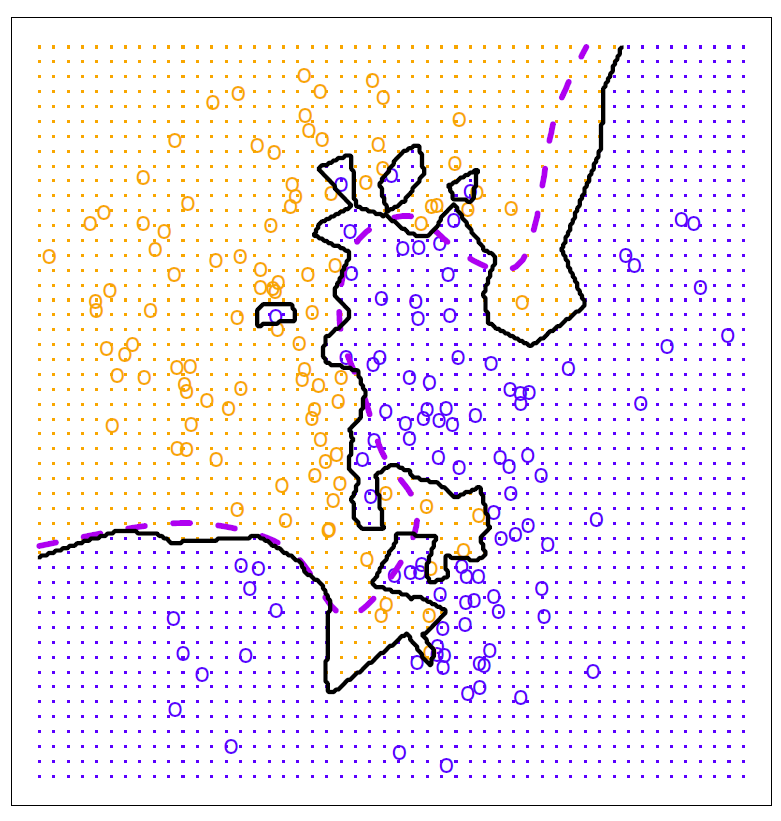
\includegraphics[width=0.8\linewidth]{knn_1.png}
\end{center}
\end{multicols}
\newpage

\part Which of the following is\textbf{ NOT} an assumption of linear regression model?

\begin{oneparchoices}
 \choice There exists a linear relationship between the predictors and the response variable.\\
 \choice The variance of error term is a constant.\\
 \choice The error term is uncorrelated across the observation.\\
 \choice The expected means of the error term is zero.\\
 \choice The least squares method is an unbiased estimation method for linear regression.
\end{oneparchoices}

\part Which of the following statements is \textbf{NOT} true?

\begin{oneparchoices}
 \choice In a data science project, you should always use a more flexible model than a simple model because a flexible model has a lower bias and thus make more accurate prediction.\\
 \choice For KNN regression models, the flexibility of the model decreases as the model uses more nearest neighbors in its prediction.\\
 \choice In SVM based classifier, a linear kernel is preferred over a nonlinear kernel if the data set if linearly separable.\\
 \choice A natural spline model generally has a low variance than a higher order of polynomial regression model.\\
 \choice A shrinkage method like Lasso and ridge regression is biased towards shrinking the estimated coefficients towards zero.
\end{oneparchoices}

\part Which of the following problems can \textbf{NOT} be solved by a k-fold cross-validation?

\begin{oneparchoices}
 \choice Estimate the tuning parameter $\lambda$ in the lasso method.\\
 \choice Determine the degree of polynomials in logistic regression.\\
 \choice Determine the number of principal components to be used in noise reduction.\\
 \choice Determine the turning parameter $C$ in the optimization problem for SVM classifiers.\\
 \choice Estimate the test MSE in a subsect selection medthod.
\end{oneparchoices}

\part Which of the following classifiers could have generated the decision boundary shown in
the figure below?

\begin{multicols}{2}
\begin{oneparchoices}
 \choice SVM with a radial kernel.\\
 \choice KNN.\\
 \choice LDA.\\
 \choice QDA.\\
 \choice Decision Tree.\\
\end{oneparchoices}

\begin{center}
  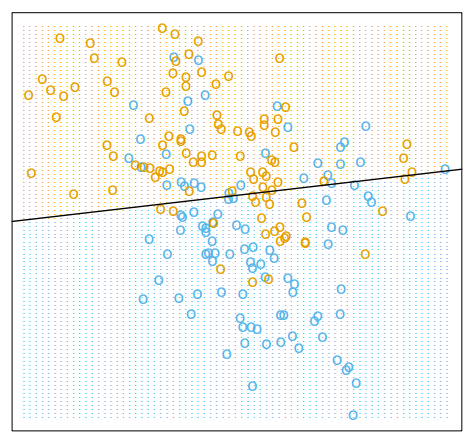
\includegraphics[width=0.8\linewidth]{lda.png}
\end{center}
\end{multicols}

\part Which of the follow statement is \textbf{FALSE}?

\begin{oneparchoices}
 \choice Given a point $\textbf{x}$ in the $p$-dimension space and a vector $\textbf{u}$ that represents the direction of a principal component, the length of the project of $\textbf{x}$ along $\textbf{u}$ is $\textbf{x} \cdot \textbf{u}/\|\textbf{u}\|^2$.\\
 \choice The principal components for a given data set aim to preserve the variance during a linear transformation. It also explains the variance of the data set.\\
 \choice PCA is susceptible to local optima.\\
 \choice PCA is an effective dimension reduction technique in regression analysis to address the curse of dimensionality problem.\\
 \choice PCA can be used for noise reduction in image preprocessing.
\end{oneparchoices}
\end{parts}
\newpage

% Question with parts
\newpage
\addpoints
\question[6] For each of the following scenarios where machine learning might be applied, indicate what machine learning algorithm you would apply and why.
\begin{itemize}
  \item You may limit the choices to those algorithms we have discussed during the class.
  \item If there are multiple proper algorithms, you can just pick up one and explain why that one is a proper one (not necessarily to the best one).
  \item Points distribution: a proper algorithm (1 point) and explaining why it is proper (2 points).
\end{itemize}

\noaddpoints
\begin{parts}
%\part[4] {\textbf{Scene Identification}}. Most cameras today allow the user to change the camera settings (ISO, shutter, speed, white balance, etc) to enhance the image quality based on the scene (Portrait,Party, night, indoors, etc). Unfortunately, the user must manually select the setting. This is far from ideal when the user tries to capture a moment but has no time or forgets to change the setting. Therefore, you would like to build software which automatically identify the type of scene and then allow the camera to automatically its settings to suit the scene. To begin with, you only consider trying to determine if an image is indoors or not. Since your company has already labelled a large collection of images as indoors and outdoors as well as extracted a compact vector representation for each image. Now you need to build a classifier which will use these vector representations and classify their corresponding images as indoors or outdoors.
%\vspace{2.5in}

\part[3] {\textbf{Document Classification}}. Your company has a large number of documents that need to be
sorted into one of three categories: Research \& Development, Finance, or Marketing. A staff at the CIO office has been able to identify a number of phrases which are commonly used in these documents. These phrases may help categorize the documents. However, there are a large number (thousands) of these phrases and each one only appears in a small number of documents. The staff has also labeled a few hundred of the documents. Now you are asked to develop a machine learning method to automatically label the rest.
\vspace{2.5in}



\part[3] {\textbf{Neighborhoods Identification}}. Your friend wants to open an Asian restaurant in Atlanta and ask your help to identify a best location to open the restaurant. You and your friend both know that the best areas to run a restaurant are those locations which have the highest Asian population and in which the top common venues visited by the public include restaurants. Assume you have already created a Atlanta city data database. You database contains a directory of all neighborhoods (name, demographical distribution of the population) in Atlanta and a directory of all business venues (name, category, neighborhood, etc.) in Atlanta. Now, you want to build machine learning software that categorizes the neighborhoods into similar groups.
\vspace{2.5in}

\end{parts}
\newpage
% If you want the total number of points for a question displayed at the top,
% as well as the number of points for each part, then you must turn off the point-counter
% or they will be double counted.

\newpage
\addpoints
\question[20] Table~\ref{credit_data} shows the first two rows of a preprocessed credit data set. This question is related to applying regression analysis to this data set.
\begin{table}[h]
  \centering
  \caption{The credit card data set.}\label{credit_data}
  \begin{tabular}{c l  l l c c c c c c l}
    \hline
    & Income &	Limit & Rating & Cards& Age & Education & Gender & Student & Married & Balance\\
\hline
1	& 14.891	& 3606	& 283	& 2	& 34	& 11 &	1	& 0	& 1	& 333 \\
2	& 106.025	& 6645	& 483	& 3	& 82	& 15 &	0	& 1	& 1	& 903 \\   \hline
  \end{tabular}
\end{table}


\begin{table}[h]
  \centering
  \caption{Model Coefficients from a linear regression analysis.}\label{credit_model}
  \begin{tabular}{l r r r r r r}
    \hline
	& coef	& std err	& t	 & $P>|t|$	& [0.025	& 0.975]\\
\hline
Intercept & -490.7701 & 39.562	& -12.405    & 0.000	& -568.636 &	-412.905\\
Income	& -7.5851	& 0.272	    & -27.902	 & 0.000	& -8.120 &	-7.050\\
Limit	& 0.1558	& 0.038	    & 4.049	     & 0.000	& 0.080 &	0.232\\
Rating	& 1.5754	& 0.577	    & 2.728	     & 0.007	& 0.439	& 2.712\\
Cards	& 17.1923	& 5.207	    & 3.302	     & 0.001	& 6.945	& 27.440\\
Age	    & -0.5275	& 0.344	    & -1.534     &	0.126  & -1.204	& 0.149\\
Education &	-0.1654	& 1.840	    & -0.090     &	0.928    &	-3.788	& 3.457\\
Gender	& 9.4699	& 11.324	& 0.836	     & 0.404	& -12.818	& 31.758\\
Student	& 423.2841	& 19.934	& 21.234     &	0.000 &	384.050	& 462.518\\
Married	& -9.3162	& 11.751	& -0.793     &	0.429 & -32.445	& 13.813\\
\hline
  \end{tabular}
\end{table}
\noaddpoints

\begin{parts}
\part[3] When apply multiple linear regression to the credit set to the training set and test set for multiple times, you observe that the mean training $R^2$ is $0.955$, the mean test $R^2$ is $0.951$, and the standard variances of both measures are very small. How do you explain this result (consistently high prediction accuracy measures which are statistically equivalent for both the training set and test set?
\vspace{2in}

\part[3] Based on the model coefficients in Table~\ref{credit_model}, \textbf{which predictor(s)} can be excluded from the linear regression model with little or no effect on the prediction accuracy and \textbf{why}?
\vspace{1in}
\newpage


%\part[2] Based on Table~\ref{credit_model} and your answer in (b), write down the regression model for balance prediction.
%\vspace{1in}



Much like the best subset selection, the lasso performs variable selection. In you analysis, you have tested the following four lasso models:
\begin{verbatim}
models = {}
models['lasso-default'] = Lasso(max_iter=5000)
models['lasso-normalized'] = Lasso(max_iter=5000, normalize=True)
models['lassoCV-default'] = LassoCV(max_iter=5000)
models['lassoCV-normalized'] = LassoCV(max_iter=5000, normalize=True)
\end{verbatim}

\begin{table}[h]
  \centering
  \caption{Coefficient estimates and model performance}\label{lasso_model}
\begin{tabular}{lrrrr}
  \hline
     & lasso-default & lasso-normalized & lassoCV-default & lassoCV-normalized\\
\hline
alpha &1.0 &1.0&872.77 & 0.059\\
Intercept &	-491.80 &	-427.35 &	-351.44 &	-488.94\\
coef. Age&-0.52& -0.0 & -0.0 & -0.47\\
coef. Cards&16.35&0.0&0.0&16.32\\
coef. Education&-0.0&0.0&0.0&-0.0\\
coef. Gender&5.24&0.0&-0.0&7.19\\
coef. Income&-7.58 &-5.18 &-5.23&-7.44\\
coef. Limit&0.15&0.08&0.23 &0.15\\
coef. Married&-5.89&-0.0&-0.0&-7.86\\
coef. Rating&1.62&2.15&0.0&1.57\\
coef. Student&410.60&351.91&0.0&418.96\\
train $R^2$&0.95&0.93&0.86&0.95\\
test $R^2$&0.96&0.92&0.84&0.95\\
train MSE&9177.22&12854.62&26889.63&9171.23\\
test MSE&11080.05&19275.55&39044.841&11238.40\\
\hline
\end{tabular}
\end{table}

\part[2] From the coefficient estimates from the lasso-normalized model, we can write the following regression model for balance prediction:
$$Balance = -427.35 - 5.18 \times Income + 0.08 \times Limit + 2.15 \times Rating + 351.91 \times Student + \epsilon $$
Which of the following interpretations of the model is (are) correct?

\begin{oneparchoices}
 \choice Every \$1,000 increase in Income is associated with an average \$5.18 decrease in balance.\\
 \choice The average balance for students is \$351.91.\\
 \choice On average, the balance of a student is \$351.91 more than that of a non-student.\\
 \choice There is no relationship between balance and limit because the coefficient for the limit is so small.
\end{oneparchoices}
\vspace{0.2in}

\part[2] Based on Table~\ref{lasso_model}, does marriage status have any effect on the balance? If yes, on average, does marriage lead to
balance increase or decrease?
\vspace{0.5in}

\newpage
\part[3] Write down the constrained optimization problem for the lasso and explain how the lasso is connected to the best subsection selection.
\vspace{2.5in}


\part[5] As a general trend, the training MSE decreases monotonically as the model flexibility increases, and there is a U-shape in the test MSE. The U-shape observed in the test MSE curves turns out to the be result of two competing properties of statistical leaning methods: variance and bias. Using the lasso as example, discuss how bias, variance, and MSE vary with the tuning parameter $\lambda$.
\vspace{4in}

\part[2] List one regression model that can output the feature importance as a by-product of its regression analysis.

\newpage
\end{parts}


\addpoints
\question[16] Consider the Default data in which the first 4 samples are shown in the table below. We are interested in creating a model to predict whether an individual will default ($Y$) on his or her credit card payment, on the basis of monthly credit card balance ($X_1$), annual income ($X_2$) and student status ($X_3$).

\begin{table}[h]
  \centering
  \caption{The Default data set}\label{balance_data}
  \begin{tabular}{crrcc}
      & balance & income & student[Yes] & default \\
      \hline \hline
    1 & 729.53 & 44361.63 & 0 & No \\
    2 & 817.18 & 12106.13 & 1 & No \\
    3 & 1073.55 & 35704.49 & 0 & No \\
    4 & 2529.25 & 38463.50 & 0 & Yes \\
    \hline
  \end{tabular}

\end{table}

\noaddpoints
\begin{parts}

\part[2] Explain why a simple linear regression model is not appropriate for the task of predicting the default using the predictors $X_1, X_2$ and $X_3$.
\vspace{1.5in}

\part[2] Write the logistic regression model for predicting the default using the three predictors $X_1, X_2$ and $X_3$. You can use $\beta_{i}$ to represent the model coefficient for the feature $X_i$.
\vspace{1.5in}


\part[2] The textbook mentioned that the coefficient of the logistic regression model can be estimated using a method called \textbf{maximum likelihood}, which essentially finds the set of coefficients that maximize a likelihood function. Write down the likelihood function for the logistic regression model you chose in (b).
\vspace{1.8in}



\newpage
For the question described above, you have estimated the logistic regression model using the following Python code and the results are shown in Table~\ref{Default_model}.

\begin{verbatim}
# Python code to estimate the logistic regression model
import statsmodels.api as sm

X = default_df[['balance', 'income', 'student[Yes]']]
y = default_df['default'].factorize()[0]
X_train = sm.add_constant(X.values)
model = sm.Logit(y, X_train).fit()
model.summary2().tables[1]
\end{verbatim}


\begin{table}[h]
  \centering
  \caption{The estimated coefficient of the logistic regression model for the Default data set.}\label{Default_model}
  \begin{tabular}{lrrrrrr}
  \hline
    & Coef.	& Std.Error.	& z	& P-value\\
    \hline
const & -10.869045 & 0.492273	& -22.08 \\
X1	& 0.005737	& 0.000232	& 24.74 \\
X2	& 0.000003	& 0.000008	& 0.37 \\
X3	& -0.646776	& 0.236257	& -2.74 \\
    \hline
  \end{tabular}

\end{table}

For the following two question, if you don't have a calculator, you can write down the formula. You will receive the partial credit if your formula is correct.

%\part[2] Using the above estimated model to predict the probability of default for a \textbf{student} with a credit card balance of \$2,000 and an income of \$38,000.
%\vspace{1.5in}


\part[2] Using the above estimated model to predict the probability of default for a \textbf{non-student} with a credit card balance of \$2,000 and an income of \$38,000.
\vspace{1.5in}

\begin{table}[h]
  \centering
  \caption{A confusion matrix comparing the LDA predictions to the true default status.}\label{Confusion_table}
  \begin{tabular}{|l|c|c|c|c|}
  \hline
  \multicolumn{1}{|}{} & \multicolumn{1}{}{} & \multicolumn{2}{|c}{True Default Status} & \multicolumn{1}{|c|}{} \\ \cline {3-5}
  \multicolumn{1}{|}{} & & \multicolumn{1}{c|}{No} & \multicolumn{1}{c|}{Yes} & Total \\
  \hline
  \multirow{3}{*}{Predicted Default Status} & \multicolumn{1}{c|}{No} & 9,644 & 252 & 9,896\\ \cline{2-5}
  & \multicolumn{1}{c|}{Yes} & 23 & 81 & 104 \\ \cline{2-5}
  & Total  & 9,667 & 333 & 10,000 \\ \hline
\end{tabular}
\end{table}

\part[2] Using the above confusion matrix, calculate the accuracy and sensitivity of the LDA classifier?
\vspace{1.6in}
\newpage

\part[3] Consider the above confusion matrix, explain why LDA does such a poor job of classifying the customers who default? How do you improve the prediction performance by making a small change on how LDA makes the classification decision?
\vspace{3.5in}


\part[3] Unlike logistic regression, LDA is linked to Bayes's Theorem and derives a discriminant function from the posterior probability that an observation belongs to a certain class based upon two major assumptions. What are the two assumptions of LDA?
\vspace{3in}

\end{parts}
\newpage

\addpoints
\question[18] \textbf{Email Spam Prediction}. We have the following email spam prediction data set. The data set comprises of three features--suspicious words ($X_1$), unknown senders ($X_2$), contains images ($X_3$)--and a class label ($Y$) (spam or ham). This question tests Naive Bayes and decision tree classifiers for the email spam prediction problem.

\begin{table}[h]
  \centering
  \caption{An email spam prediction data set}\label{email_spam_data}
  \begin{tabular}{ccccc}
    \hline
    % after \\: \hline or \cline{col1-col2} \cline{col3-col4} ...
    ID & Suspicious Words & Unknown Senders & Contains Images & Class \\
    \hline
    376 & true & false & true & spam \\
    489 & true & true & false & spam \\
    541 & true & true & false & ham \\
    693 & false & true & false & ham \\
    782 & false & false & false & ham \\
    976 & false & false & false & ham \\
    \hline
  \end{tabular}
\end{table}

\noaddpoints
\begin{parts}
\part[2] Apply the Bayes's theorem to the email spam problem, we have the following equation $$P(Y=l|X_1,X_2,X_3) = \frac{P(X_1,X_2,X_3|Y=l) \times P(Y=l)}{P(X_1, X_2, X_3)}$$
In this equation, which term is the likelihood, prior probability, and posterior probability?

\vspace{0.1in}
\begin{table}[h]
  \centering
  \begin{tabular}{l|c}
    \hline
    % after \\: \hline or \cline{col1-col2} \cline{col3-col4} ...
    Term & Write the Appropriate Term Name in this Column \\
    \hline
    & \\
    $P(Y=l|X_1,X_2,X_3)$ & \\
    & \\
    \hline
    & \\
    $P(X_1,X_2,X_3|Y=l)$ & \\
    & \\
    \hline
    & \\
    $P(Y=l)$\\
     & \\
    \hline
    & \\
    $P(X_1, X_2, X_3)$\\
    &\\
    \hline
  \end{tabular}
\end{table}
\vspace{0.1in}
\part[2] A probability based statistical learning methods relies on estimations of several probabilities appeared in the Bayes's theorem. What are the two fundamental principles (i.e. methods) for probability estimation?
\vspace{2in}
\newpage

\part[4] Naives Bayes uses the production rule $$P(X_1,X_2,\ldots,X_p|Y=l) = \prod_{i=1}^pP(X_i|Y=l)$$ to compute the conditional joint probability $P(X_1,X_2,\ldots,X_p|Y=l)$. Prove that the production rule holds under the conditional independence assumption on the predictors.
\vspace{3.6in}


\part[3] Using the production rule and the Bayes' Theorem to compute the probability $$P(\texttt{Y=spam|Suspicious~Words=true, Unknown~Senders=false, Contains~Image=true})$$
In your computation, you can assume
$$P(\texttt{Suspicious~Words=true, Unknown~Senders=false, Contains~Image=true}) = \frac{1}{6}$$

\newpage

\part[5] A decision tree classifier recursively splits the data set into sub data sets using the features that gives the maximum information gain.\textbf{ Compute the information gain }obtained by splitting the data based on the \textbf{Suspicious Words} feature. In this question, assume the information measure is Shannon's entropy. For your reference, below are the equations to compute the entropy of a data set and the remainder after split using a feature.
$$H(y, D)=-\sum_{l\in Classes(y)} P(y=l)log_2(P(y=l))$$.
$$Rem(d, D)=-\sum_{l \in Classes(d)} \frac{\|D_{d=l}\|}{\|D\|} \times H(y, D_{d=l})$$.
\vspace{5in}


\part[2] A decision tree classifier suffers from high variance, i.e., different training set can result in different trees. Provide a learning method that has lower variance in comparison with the decision tree classifier.

\newpage
\end{parts}

\newpage

\addpoints
\question[10] This question tests your understanding of SVM.
\noaddpoints
\begin{parts}
\part[2] Give a data set shown in Figure below, draw the separating hyperplane resulted from an SVM classifier and circle all the support vectors.
\begin{figure}[h]
  \centering
  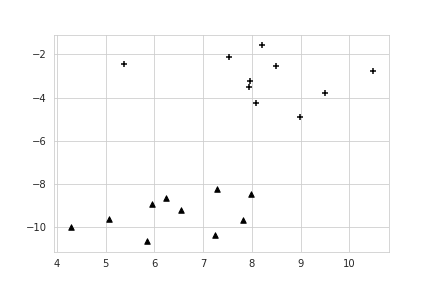
\includegraphics[width=0.65\linewidth]{svm_data.png}
  %\caption{A simulated data set}\label{svm-data}
\end{figure}
\vspace{0.2in}

\part[2] The plots below show a Support Vector Classifier that was fit on the same data using four different
values for the tuning parameter $C$. Which of the classifiers has the smallest bias but potentially
largest variance?
\begin{figure}[h]
  \centering
  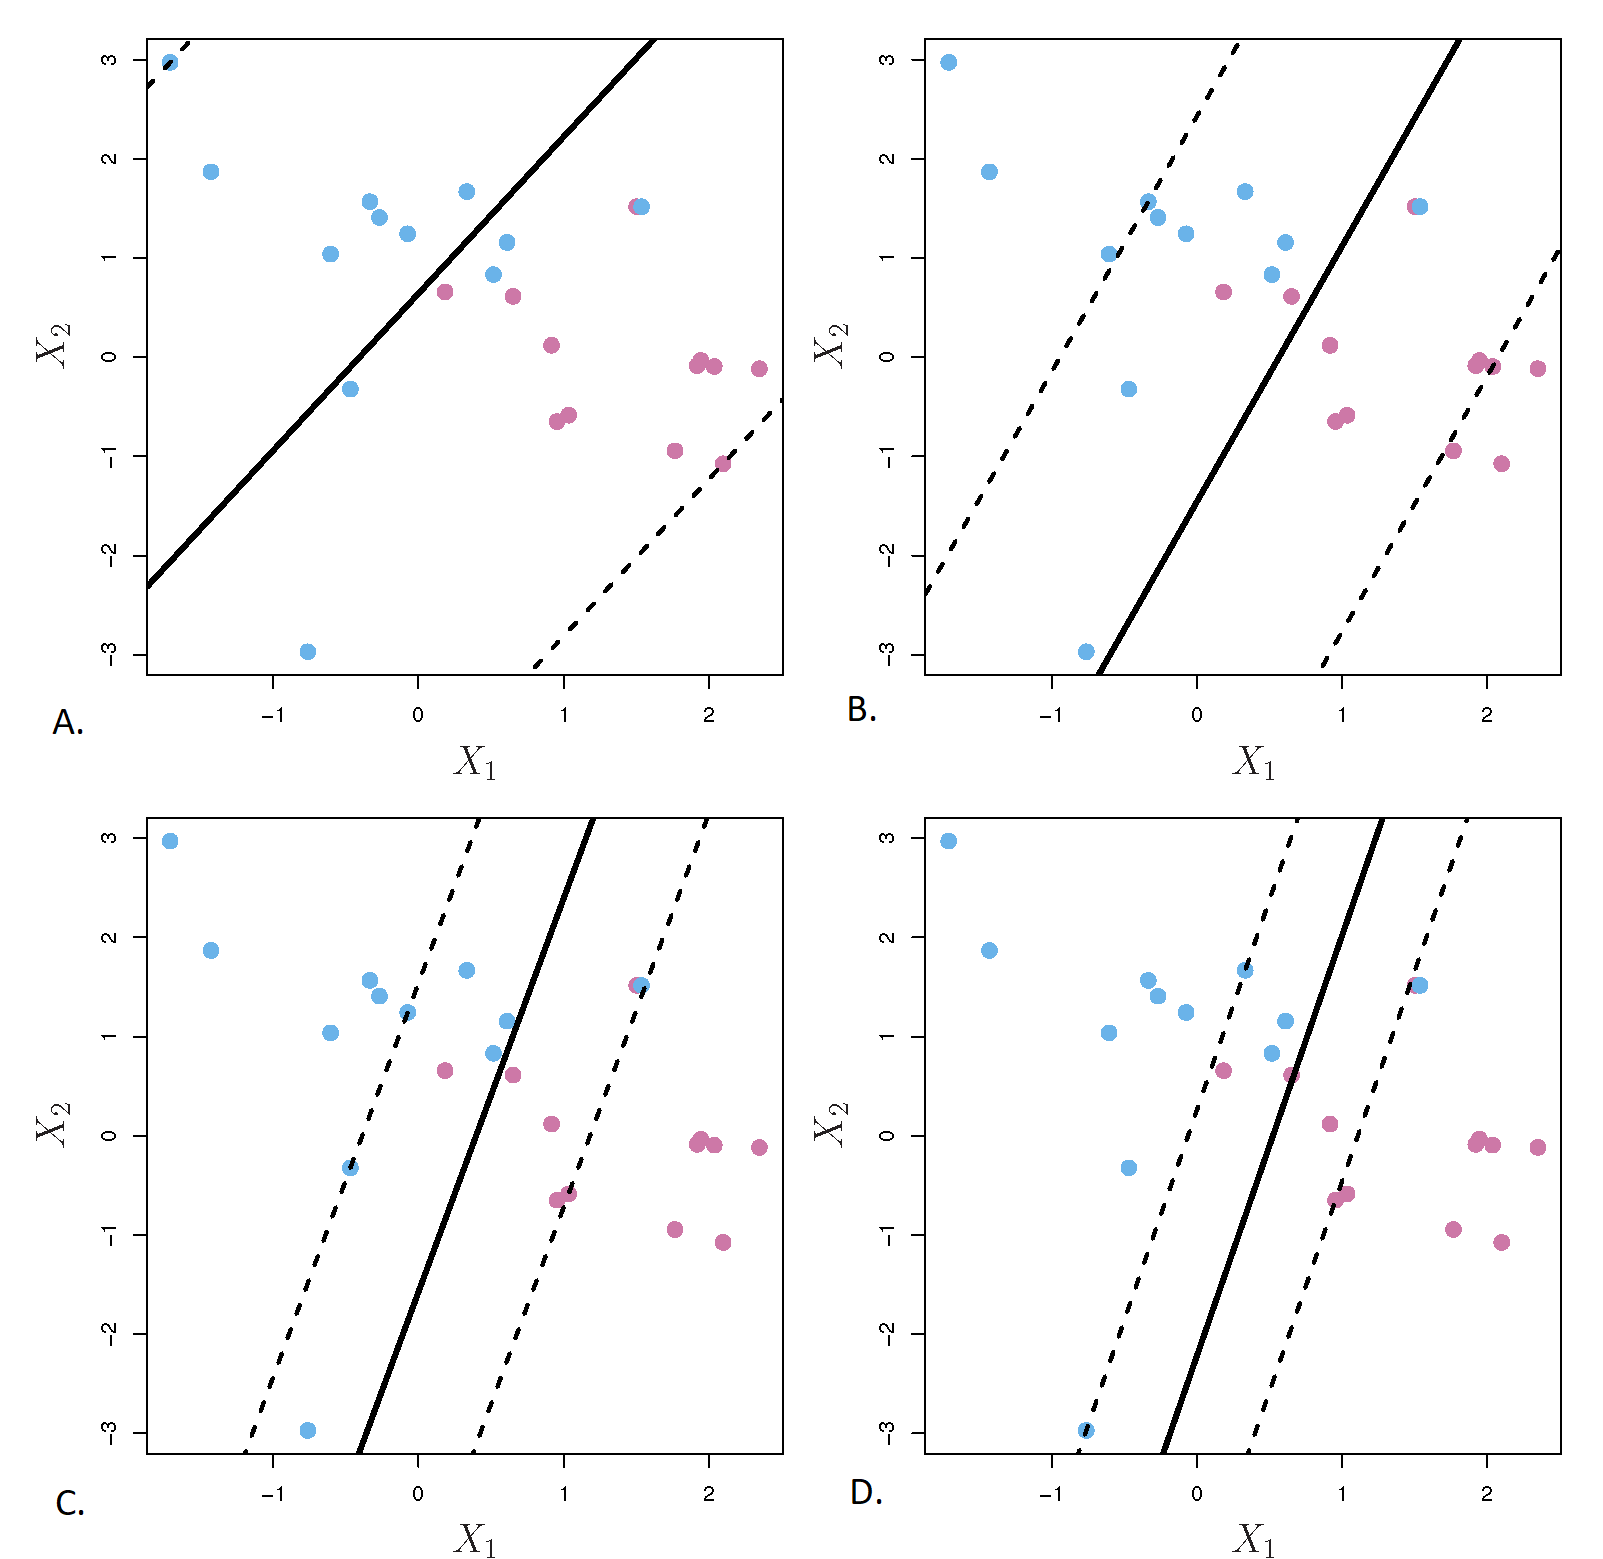
\includegraphics[width=0.6\linewidth]{svc_turing.png}
  %\caption{A simulated data set}\label{svc-turning}
\end{figure}
\vspace{0.2in}

\part[3] Show that $K(u,v)=(u^ T\cdot v + 1)^2$ is a kernel that corresponds to the mapping $\phi: x \mapsto (x^2, \sqrt{2}x, 1)^T$, where $x$, $u$ and $v$ are all vectors in $1$D space. In other words, show $K(u, v) = \phi(u)^T \cdot \phi(v)$.
\vspace{3.3in}

\part[3] In the figure below, sketch the corresponding images (i.e., $\phi(x)$ for point $x$) of the points A-E in the 1D space in the 2D space using the mapping $\phi: x \mapsto (x^2, \sqrt{2}x)^T$. \textbf{In the 2D space}, sketch the separating hyperplane and circle all the support vectors.
\begin{figure}[h]
  \centering
  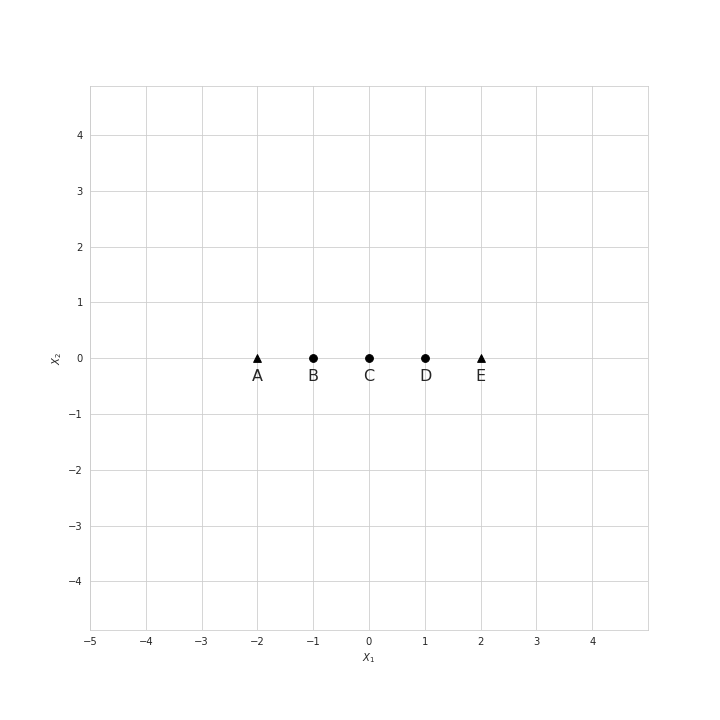
\includegraphics[width=0.65\linewidth]{svm_kernel.png}
  %\caption{A simulated data set}\label{svm-data}
\end{figure}
\end{parts}


\newpage
\addpoints
\question[15] This problem tests your understanding of the \textbf{$K$-Means Clustering}.

\begin{parts}
\noaddpoints
\part[2] Generally an unsupervised learning algorithm aims to solve an optimization problem. What objective function does a $K$-means clustering seek to minimize?
\vspace{1.5in}


\part[3] Sketch the $K$-means algorithm below and mark the key steps and termination condition(s).
\vspace{4.5in}

\part[3] Does the $K$-means algorithm always converge? Explain why?
\vspace{1.5in}
\newpage

\part[4] In this problem, you will perform $K$-means clustering manually, with $K = 2$, on a small data set with $n = 5$ observations and $p = 2$ features. The observations are as follows.

\begin{table}[h]
  \centering
  \begin{tabular}{c|c|c}
  \hline
  Obs. & $X_1$ & $X_2$ \\
  \hline
  1 & 1 & 4 \\
  2 & 1 & 3 \\
  3 & 0 & 4 \\
  4 & 5 & 1 \\
  5 & 4 & 0 \\
  \hline
\end{tabular}
\end{table}

You label the two clusters with \textbf{$+$} and \textbf{$-$}. In a particular run of the $K$-means algorithm, you assign observation 1 to cluster \textbf{$+$} and observation 2 to cluster \textbf{$-$}.

\begin{subparts}
\subpart In the following table, assign a cluster label to all the observations.

\begin{table}[h]
  \centering
  \begin{tabular}{c|c|c|c}
  \hline
  Obs. & $X_1$ & $X_2$ & Cluster\\
  \hline
  1 & 1 & 4 & \textbf{$+$} \\
  2 & 1 & 3 & \textbf{$-$} \\
  3 & 0 & 4 & \\
  4 & 5 & 1 & \\
  5 & 4 & 0 & \\
  \hline
\end{tabular}
\end{table}
\vspace{0.3in}

\subpart after step i, the coordinates of the new centroid for cluster \textbf{$+$} will be
\\
\\
 (\fillin, \fillin).
\vspace{0.3in}

\end{subparts}


\if false
\part[2] The $K$-means algorithm will generally converge to a local optima rather than a global one. Given this, how would you adapt the algorithm to increase the chances of finding
a good solution?
\vspace{1.0in}
\fi


\part[3] List three caveats of the k-means algorithm.
\vspace{1.5in}

\end{parts}

\newpage

\newpage
\end{questions}
\end{document} 